\section{Graphical User Interface}

This section contains a beta version of the system's graphical user interface (GUI).

When the user opens the GUI, the main window, shown in Figure~\ref{fig:mainWindow}, is shown. The user needs to select a sphere in order to perform any other action.  Figure~\ref{fig:viewSphere} shows the information and options available when a sphere is selected. From this screen, the user can select to operate the sphere in several modes including retrieval, sampling and diagnostic modes.  The user can also choose to send a signal to turn on or off the selected sphere.
\begin{figure}[H]
	\centering
	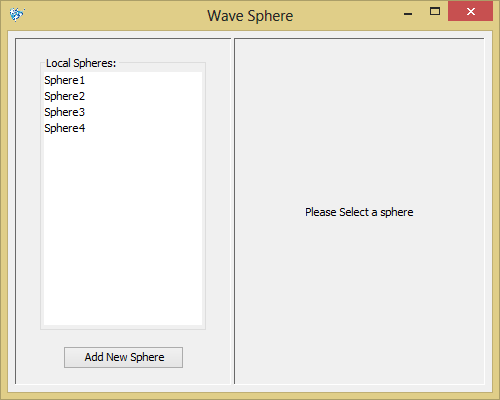
\includegraphics[scale=0.7]{img/mainWindow}
	\caption{Main Window \label{fig:mainWindow}}
\end{figure}

\begin{figure}[H]
	\centering
	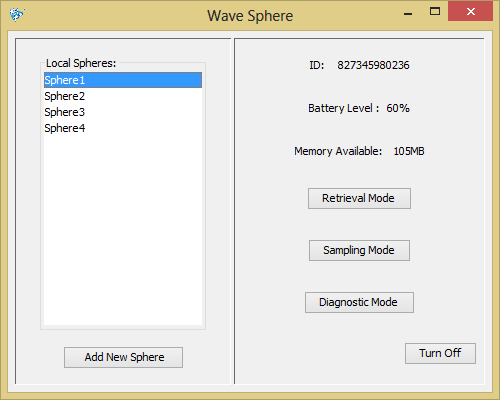
\includegraphics[scale=0.7]{img/viewSphere}
	\caption{Sphere View \label{fig:viewSphere}}
\end{figure}
When the user selects retrieval mode, the right section of the GUI changes, as shown in Figure~\ref{fig:retrievalMode}, to allow the user to retrieve the data collected by the selected sphere.  When the user selects one of the download options the GUI asks for the location where the user wants to store the data, as shown in Figure~\ref{fig:download}. 
\begin{figure}[H]
	\centering
	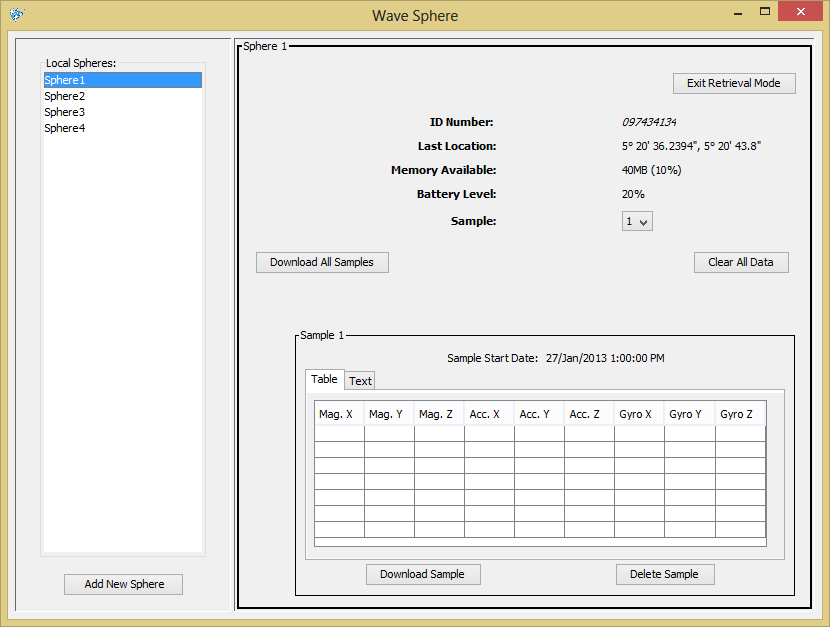
\includegraphics[scale=0.7]{img/retrievalMode}
	\caption{Retrieval Mode \label{fig:retrievalMode}}
\end{figure}

\begin{figure}[H]
	\centering
	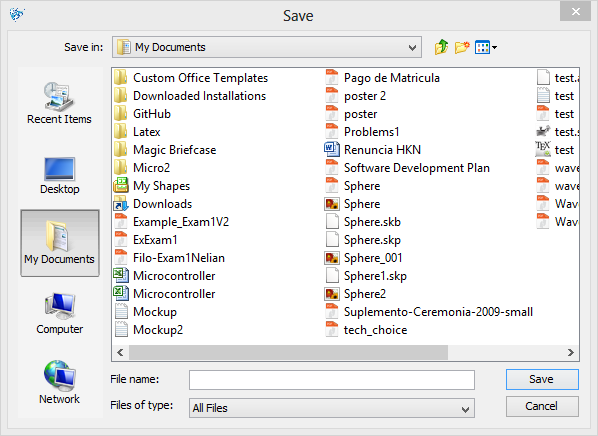
\includegraphics[scale=0.7]{img/download}
	\caption{Download \label{fig:download}}
\end{figure}

When the user selects sampling mode, a progress bar will be shown to indicate the time elapsed and remaining throughout duration of the sample. Figure~\ref{fig:samplingMode} shows how the window looks in this mode. After the data sampling is completed, the GUI automatically enters locate mode and opens a pop-up to show location information, as shown in Figure~\ref{fig:locateMode}.  When the user exits locate mode, they are directed to the "Sphere View" shown in Figure~\ref{fig:viewSphere}.
\begin{figure}[H]
	\centering
	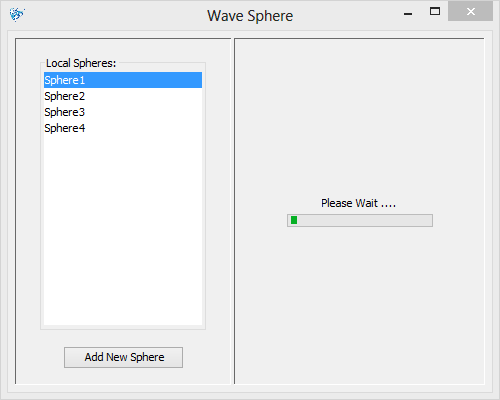
\includegraphics[scale=0.7]{img/samplingMode}
	\caption{Sampling Mode \label{fig:samplingMode}}
\end{figure}

\begin{figure}[H]
	\centering
	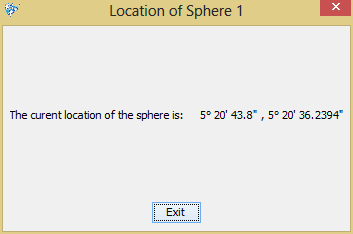
\includegraphics[scale=0.7]{img/locateMode}
	\caption{Locate Mode \label{fig:locateMode}}
\end{figure}

When the user selects diagnostic mode, a pop-up showing diagnostic information appears, as shown in figure~\ref{fig:diagnosticMode}.  This will allow the user to ensure the proper operation of the selected sphere.

\begin{figure}[H]
	\centering
	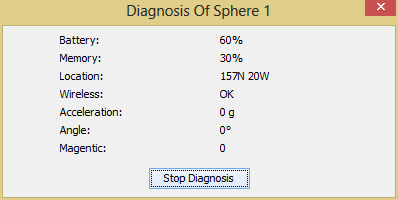
\includegraphics[scale=0.7]{img/diagnosticMode}
	\caption{Diagnostic Mode \label{fig:diagnosticMode}}
\end{figure}